\chapter{Sniffer}
\section{Sniffeo de la red}
La primera parte del trabajo, consisti� en la implementaci�n de un sniffer, el cual deb�a escuchar el tr�fico que se dirige a un proxy y guardar en una base de datos los mensajes HTTP y otros mensajes como ser SSH, SSL, o TLS.

\begin{figure}[H]
\centering
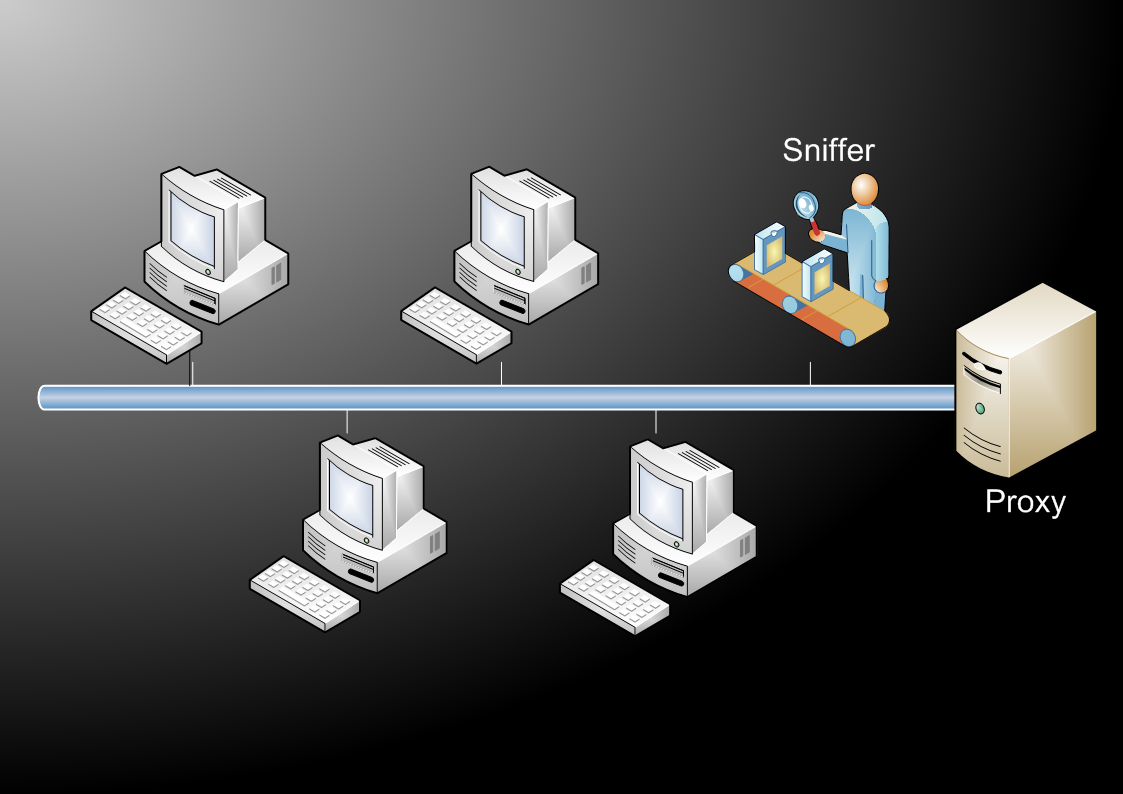
\includegraphics[scale=0.4]{./figuras/sniffer.png}
\caption{Esquema de la ubicaci�n del sniffer}
\end{figure}

Para la construcci�n del sniffer utilizamos la librer�a Scapy. Esta es una libreria para python que brinda amplias facilidades para el manejo de paquetes a nivel TCP, Ethernet, ICMP y demas. Posee ademas otras caracteristicas interesantes, como la capacidad de generar traceroutes.

Scapy provee una forma de sniffear trafico en una interfaz de red. Utilizando esto construimos nuestro sniffer, el cual es capaz de recibir callbacks que se invocan cada vez que se recibe un nuevo paquete. Esta funcionalidad nos permite construir alrededor del sniffer no solo la funcionalidad de capturar y guardar el trafico http, sino que permite ademas construir otras funcionalidades que se consideren utiles. En nuestro caso utilizamos esta posibilidad de los callbacks para realizar dumps a archivos pcap o para ir mostrando por pantalla los paquetes que se iban capturando.

Otra caracteristica positiva de construir al sniffer de esta manera, es que permite separar el proceso de sniffear del proceso de construir los paquetes HTTP y demas, para guardarlos en la base de datos.

El siguiente es un esquema que ilustra la estructura del sniffer:

\begin{figure}[H]
\centering
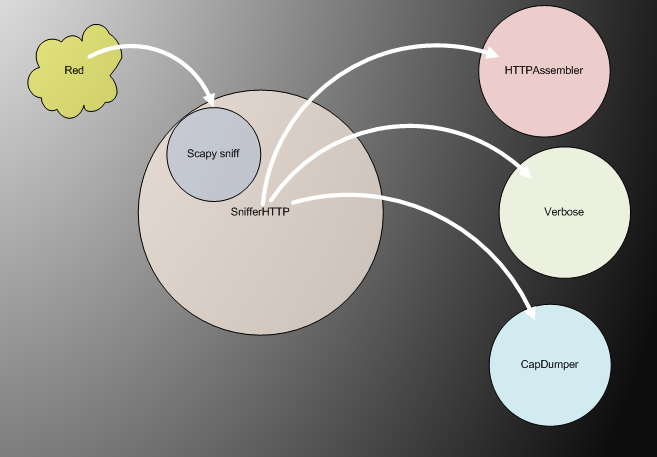
\includegraphics[scale=0.7]{./figuras/esquemaSniff.png}
\end{figure}

En el esquema vemos que utilizando las capacidades de scapy para hacer sniff logramos capturar los paquetes, que luego nuestro sniff pasa a sus suscriptores mediante los callbacks que estos  registran.

\section{Mensajes HTTP}
Cuando se detecta un paquete que llega al puerto del proxy, el mismo pasa a ser examinado. Del paquete se extrae el contenido (o capa RAW), si no hay contenido RAW (por ejemplo se trata de un mensaje TCP SYN) no se procesa. Si el contenido es un mensajeHTTP el mismo se persiste. Si no, se chequea que el mensaje sea el comienzo de un mensaje HTTP y si es asi se crea un estado para la cuadrupla propia de esa conexi�n TCP, donde se van a ir agregando el contenido de los paquetes que lleguen de esa conexi�n, hasta tener el mensaje HTTP completo. Es posible que el mensaje HTTP llegue partido porque TCP no se preocupa por eso sino que es responsabilidad de la aplicaci�n saber cuando terminan sus datos, y como nosotros estamos escuchando la red, vamos a tener que ser nosotros quienes rearmen el mensaje.

Entre los posibles mensajes que se pueden escuchar, hay requests cuyo metodo  es CONNECT. Estos en general se usan antes de comenzar una conexi�n SSH, TLS, o SSL. Entonces cuando se detecta una CONNECT, se empieza a escuchar ese trafico para detectar si se trata de trafico no HTTP. En caso afirmativo el trafico de la conexi�n se persiste. Notar que a esta altura solo diferenciamos trafico HTTP, de trafico no HTTP. La discriminaci�n entre otros protocolos de aplicaci�n es posterior.

\section{Otras caracteristicas de sniffer}
Ademas de sniffear trafico HTTP y persitirlo, la aplicaci�n brinda otras funcionalidades, entre ellas:

\begin{itemize}
\item Dumpeo de la sesi�n de captura a un archivo pcap. Esto es util si se quiere analizar en otra herramienta las capturas realizadas. El arhivo generado contiene todos los paquetes capturados, no solo lo que es trafico HTTP.
\item Simulaci�n de una sesi�n de captura a partir de un archivo pcap. El sniffer puede simular una captura en vivo mediante un archivo pcap. Esto es util si se realizan capturas con otro sniffer como el wireshark, y se desea poder analizar a la misma con la herramienta de reportes que presentaremos mas adelante y que corresponde a la segunda parte del trabajo
\end{itemize}

Ademas, dado que se utiliza un dise�o basado en callbacks, es facil extender las funcionalidades del sniffer, simplemente definiendo una clase y suscribiendo un metodo de la misma que realice las manipulaciones deseada al paquete.

%TODO: tal vez un ejemplo de esto?

\section{Algunas limitaciones}
Nuestro sniffer presenta algunas limitaciones, creemos que las mas importantes son:

\subsection*{Performance}
Si bien creemos que python es un gran lenguaje y muy flexible, somos conscientes que su performance dista de la que se puede lograr programando en C, ademas pudimos averiguar que scapy puede perder paquetes si la carga es muy grande \footnote{http://www.secdev.org/projects/scapy/}. Si bien no pudimos probar al sniffer con una carga muy grande, creemos que es factible que la performance sea un limitante para su uso.

\subsection*{Consideraciones de seguridad}
Basicamente el sniffer no fue hecho para correr en ambientes hostiles. As� por ejemplo creemos que es factible que un usuario malicioso logre generar una denegaci�n de servicio, generando la caida del sniffer. Esto se debe a que como comentamos antes, cuando llega un fragmente de mensaje HTTP se guarda cierta informaci�n de estado para poder armar todo el mensaje. 


\begin{figure}[H]
\centering
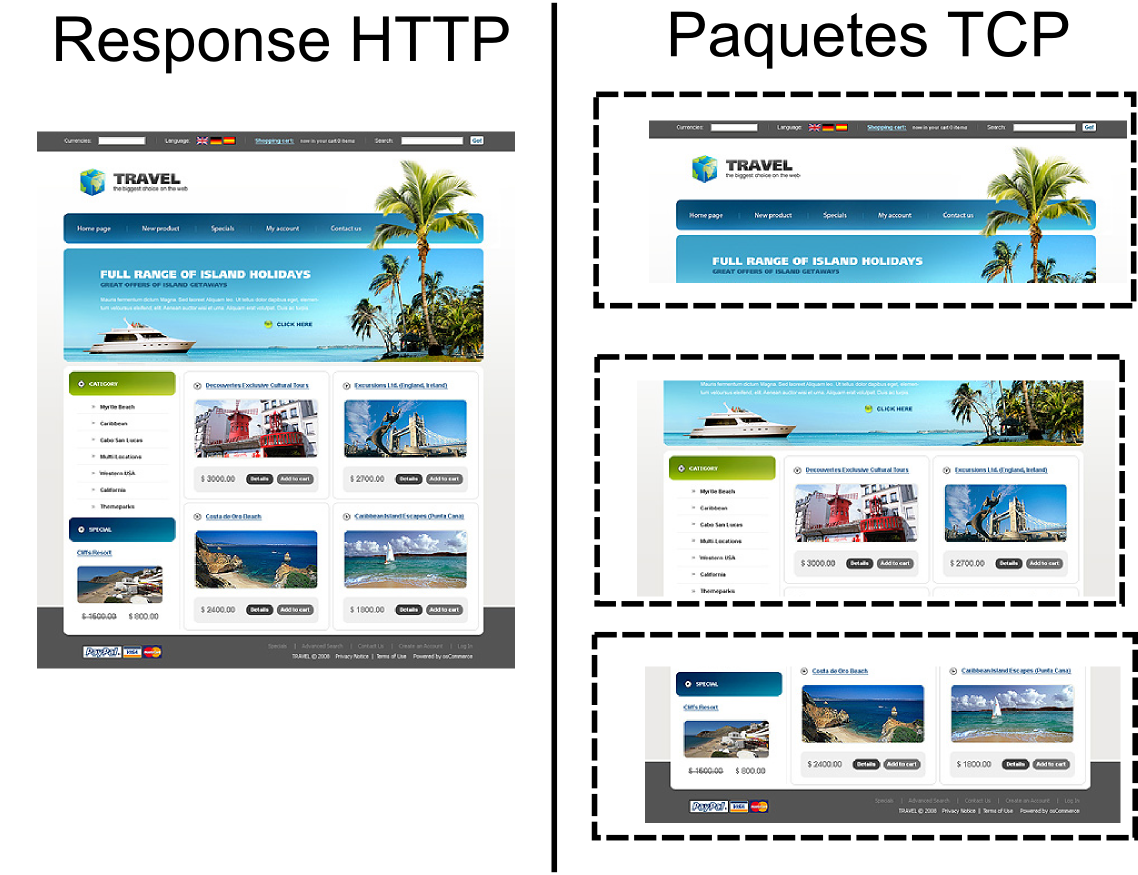
\includegraphics[scale=0.3]{./figuras/fragTCP.png}
\caption{Un mensaje HTTP puede venir fragmentado en varios mensajes TCP}
\end{figure}

Entonces un usuario malicioso puede enviar una gran cantidad de mensajes inconclusos y el sniffer, al guardar la informaci�n de estado de estos, termina agotando sus recursos. Esta situaci�n es similar a lo que ocurre con un ataque de \textit{SYN flooding} en TCP. 

\begin{figure}[H]
\centering
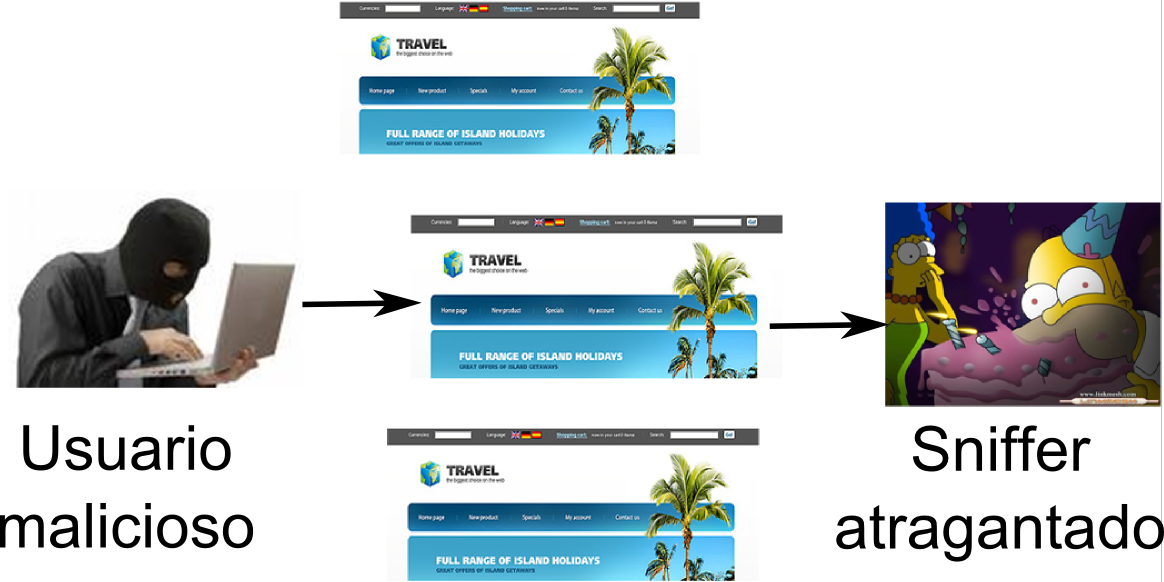
\includegraphics[scale=0.4]{./figuras/atraganta.png}
\caption{Al enviar muchos paquetes inconclusos, un usuario malicioso podr�a lograr agotar los recursos del sniffer}
\end{figure}


Esta vulnerabilidad no fue probada, sin embargo la consideramos altamente factible de explotar.



